\subsection{UC1 – Utente Non Autenticato}

\subsubsection{UC1.1 – Registrazione}
\begin{center}
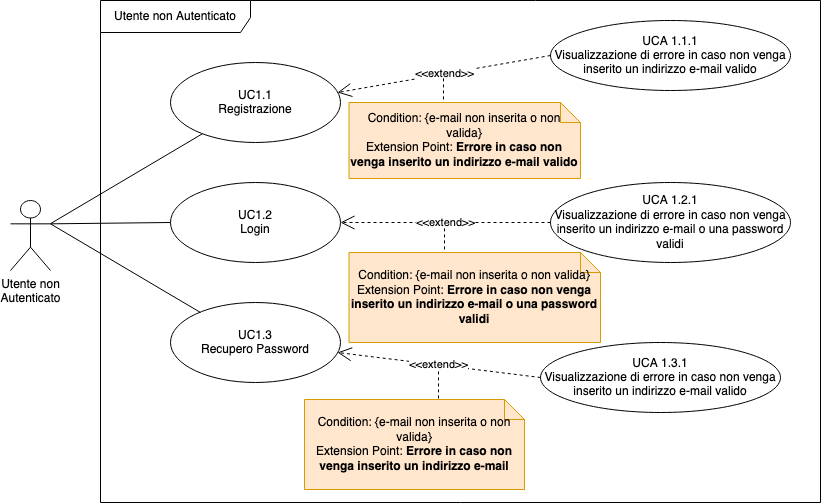
\includegraphics[scale=0.5]{UC_images/UC1.png}
\end{center}
\begin{itemize}
\item \textbf{Attore primario}: Utente non autenticato.
\item \textbf{Precondizione}: L'utente non è ancora autenticato presso il sistema.
\item \textbf{Postcondizione}: L’utente possiede un account con cui può accedere al sistema, contraddistinto da una username ed una password.

\item \textbf{Scenario principale}:
\begin{enumerate}
\item L’utente accede al sistema;
\item L’utente seleziona la funzionalità “Registrati”;
\item L'utente inserisce i campi dati obbligatori: Nome e Cognome;
\item L’utente inserisce un indirizzo e-mail univoco nel campo username non ancora utilizzato con cui accedere al sistema; 
\item L’utente inserisce una password per accedere al sistema;
\item Affinché la registrazione vada a buon fine, l’utente dovrà cliccare su “Registrati”.
\end{enumerate}

\item \textbf{Estensioni}:
\begin{itemize}
\item Nel caso in cui l’utente inserisca un indirizzo e-mail non esistente, già presente a sistema o lasci il campo vuoto
\begin{enumerate}
	\item L’utente non viene registrato nel sistema;
	\item Viene mostrato un messaggio d’errore che indica che l'indirizzo e-mail inserito non è corretto (UC1.1.1 §).
\end{enumerate}
\item Nel caso in cui l’utente provi a registrarsi inserendo una password più breve di 8 caratteri
\begin{enumerate}
	\item L’utente non viene registrato nel sistema;
	\item Viene mostrato un messaggio d’errore che indica che non è stata inserita alcuna password (UC1.1.2 §).
\end{enumerate}
\item{Nel caso in cui l'utente non inserisca il proprio nome e cognome}
\begin{enumerate}
	\item L'utente non viene registrato nel sistema;
	\item Viene mostrato un messaggio d'errore che indica che il nome ed il cognome non sono stati inseriti correttamente (UC1.1.3 §).
\end{enumerate}
\end{itemize}
\end{itemize}

\subsubsection{UC1.1.1 – Errore inserimento e-mail}
\begin{itemize}
\item \textbf{Attore primario}: Utente non autenticato.
\item \textbf{Precondizione}: L'utente non è ancora autenticato presso il sistema.
\item \textbf{Postcondizione}: Viene mostrato un messaggio d'errore e l'utente non viene autenticato nel sistema.

\item \textbf{Scenario principale}:
\begin{enumerate}
\item L'operazione di inserimento dell'indirizzo e-mail fallisce;
\item Viene mostrato il corrispondente messaggio d'errore;
\item All'utente viene data la possibilità di tentare nuovamente la registrazione al sistema.
\end{enumerate}
\end{itemize}

\subsubsection{UC1.1.2 – Errore inserimento password}
\begin{itemize}
\item \textbf{Attore primario}: Utente non autenticato.
\item \textbf{Precondizione}: L'utente non è ancora autenticato presso il sistema.
\item \textbf{Postcondizione}: Viene mostrato un messaggio d'errore e l'utente non viene autenticato nel sistema.

\item \textbf{Scenario principale}:
\begin{enumerate}
\item L'operazione di inserimento password fallisce;
\item Viene mostrato il corrispondente messaggio d'errore;
\item All'utente viene data la possibilità di tentare nuovamente la registrazione al sistema.
\end{enumerate}
\end{itemize}

\subsubsection{UC1.1.3 – Errore inserimento dati personali}
\begin{itemize}
\item \textbf{Attore primario}: Utente non autenticato.
\item \textbf{Precondizione}: L'utente non è ancora autenticato presso il sistema.
\item \textbf{Postcondizione}: Viene mostrato un messaggio d'errore e l'utente non viene autenticato nel sistema.

\item \textbf{Scenario principale}:
\begin{enumerate}
\item L'operazione di inserimento dei dati personali (Nome e Cognome) fallisce;
\item Viene mostrato il corrispondente messaggio d'errore;
\item All'utente viene data la possibilità di tentare nuovamente la registrazione al sistema.
\end{enumerate}
\end{itemize}

\subsubsection{UC1.2 – Login}
\begin{itemize}
\item \textbf{Attore primario}: Utente non autenticato.
\item \textbf{Precondizione}: L'utente non è ancora autenticato presso il sistema.
\item \textbf{Postcondizione}: L’utente ha effettuato l’accesso al sistema ed è all’interno del proprio account.

\item \textbf{Scenario principale}:
\begin{enumerate}
\item L’utente accede al sistema;
\item L’utente seleziona la voce “Login”;
\item L’utente inserisce l’indirizzo e-mail con cui è registrato al sistema;
\item L’utente inserisce la password d’accesso; 
\item L’utente seleziona la voce “Login”. 
\end{enumerate}

\item \textbf{Estensioni}:
\begin{itemize}
\item Viene inserito uno username errato / non registrato
\begin{enumerate}
	\item L’utente non può accedere al sistema;
	\item Viene mostrato un messaggio d’errore che indica che lo username inserito non è corretto (UC1.2.1 §). 
\end{enumerate}
\item Viene inserita una password errata
\begin{enumerate}
	\item L’utente non può accedere al sistema;
	\item Viene mostrato un messaggio d’errore che indica che la password inserita non è corretta (UC1.2.2 §).
\end{enumerate}
\end{itemize}
\end{itemize}

\subsubsection{UC1.2.1 – Errore inserimento username}
\begin{itemize}
\item \textbf{Attore primario}: Utente non autenticato.
\item \textbf{Precondizione}: L'utente non è ancora autenticato presso il sistema.
\item \textbf{Postcondizione}: Viene mostrato un messaggio d'errore e l'utente non viene autenticato nel sistema.

\item \textbf{Scenario principale}:
\begin{enumerate}
\item L'operazione di inserimento dello username fallisce;
\item Viene mostrato il corrispondente messaggio d'errore;
\item All'utente viene data la possibilità di tentare nuovamente l'accesso al sistema.
\end{enumerate}
\end{itemize}

\subsubsection{UC1.2.2 – Errore inserimento password}
\begin{itemize}
\item \textbf{Attore primario}: Utente non autenticato.
\item \textbf{Precondizione}: L'utente non è ancora autenticato presso il sistema.
\item \textbf{Postcondizione}: Viene mostrato un messaggio d'errore e l'utente non viene autenticato nel sistema.

\item \textbf{Scenario principale}:
\begin{enumerate}
\item L'operazione di inserimento dello username fallisce;
\item Viene mostrato il corrispondente messaggio d'errore;
\item All'utente viene data la possibilità di tentare nuovamente l'accesso al sistema.
\end{enumerate}
\end{itemize}

\subsubsection{UC1.3 – Password Dimenticata}
\begin{itemize}
\item \textbf{Attore primario}: Utente non autenticato.
\item \textbf{Precondizione}: L’utente non è ancora autenticato presso il sistema.
\item \textbf{Postcondizione}: L’utente ha la possibilità di recuperare la password tramite l'indirizzo e-mail con cui è registrato nella piattaforma.

\item \textbf{Scenario principale}:
\begin{enumerate}
\item L’utente accede al sistema;
\item L’utente seleziona la voce “Login”;
\item L’utente clicca sulla voce “Password dimenticata”;
\item L’utente inserisce l’indirizzo e-mail da cui recuperare la password;
\item L’utente clicca su “Recupera password”. 
\end{enumerate}

\item \textbf{Estensioni}:
\begin{itemize}
\item Viene inserito un indirizzo e-mail non valido / non registrato
\begin{enumerate}
	\item L’utente non può recuperare la password;
	\item Viene mostrato un messaggio d’errore che indica che l’indirizzo e-mail inserito non è corretto (UC1.2.2 §).
\end{enumerate}
\end{itemize}
\end{itemize}

